\documentclass[letterpaper,10pt]{extarticle}
\usepackage[utf8]{inputenc}
\usepackage[T1]{fontenc}
\usepackage{graphicx}
\usepackage[x11names]{xcolor}
\usepackage{tikz}
\usetikzlibrary{circuits.ee.IEC}
\usepackage[os=win]{menukeys}

\usepackage{amsmath,amssymb,textcomp}
\everymath{\displaystyle}

\usepackage{physics}

\usepackage{times}
\renewcommand\familydefault{\sfdefault}
\usepackage{tgheros}
\usepackage{droidmono}

\usepackage{enumitem}
\usepackage[explicit]{titlesec}

\usepackage{multicol}
\setlength{\columnseprule}{0pt}
\setlength{\columnsep}{15.0pt}
\usepackage{multirow}
\usepackage[mode=buildnew]{standalone}

\usepackage{geometry}
\geometry{left=10mm,right=10mm,top=10mm,bottom=15mm,showframe=false}

% custom title
\makeatletter
\renewcommand*{\maketitle}{%
\noindent
\begin{minipage}{0.82\textwidth}

\begin{tikzpicture}
\node[rectangle,rounded corners=6pt,inner sep=6pt,fill=SteelBlue1,text width=.95\textwidth] {\color{black}\huge \@title};
\end{tikzpicture}
\end{minipage}
\hfill
\begin{minipage}{0.17\textwidth}
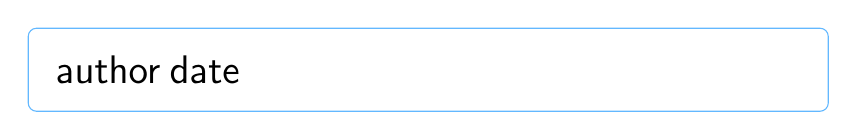
\begin{tikzpicture}
\node[rectangle,rounded corners=3pt,inner sep=10pt,draw=SteelBlue1,text width= 0.78\textwidth] {\raggedleft \Large \@author\ \@date};
\end{tikzpicture}
\end{minipage}
%\bigskip%\bigskip
}%
\makeatother

% custom section
\newcommand*\sectionlabel{}
\titleformat{\section}
  {\gdef\sectionlabel{}
   \normalfont\sffamily\Large\bfseries\scshape}
  {\gdef\sectionlabel{\thesection\ }}{0pt}
  {
\noindent
\begin{tikzpicture}
\node[rectangle,rounded corners=3pt,inner sep=4pt,fill=DodgerBlue4,text width= 0.95\columnwidth] {\color{white}\sectionlabel#1};
\end{tikzpicture}
  }
\titlespacing*{\section}{0pt}{1pt}{0.5pt}

% custom subsection
\newcommand*\subsectionlabel{}
\titleformat{\subsection}{\normalfont\sffamily\bfseries\scshape}{\subsectionlabel}{0pt}{
\noindent
\begin{tikzpicture}
\node[rectangle,rounded corners=4pt,inner sep=3pt,fill=DodgerBlue3,text width= 0.95\columnwidth] {\color{white}\subsectionlabel#1};
\end{tikzpicture}
}
\titlespacing*{\subsection}{0pt}{.5pt}{.5pt}

% custom subsubsection
\newcommand*\subsubsectionlabel{}
\titleformat{\subsubsection}{\normalfont\sffamily\small\bfseries\scshape}{\subsubsectionlabel}{0pt}{
\noindent
\begin{tikzpicture}
\node[rectangle,rounded corners=3pt,inner sep=3pt,fill=blue!50!yellow,text width= 0.95\columnwidth] {\color{white}\subsubsectionlabel#1};
\end{tikzpicture}
}
\titlespacing*{\subsubsection}{0pt}{.5pt}{.5pt}


\title{PHY335 : Physique des ondes}
\author{Examen 1}
\date{E2019}

%\linespread{1.3}

\begin{document}
\maketitle

\begin{multicols*}{2}

\setlength{\belowdisplayskip}{2.5pt}
\setlength{\belowdisplayshortskip}{2.5pt}
\setlength{\abovedisplayskip}{2.5pt}
\setlength{\abovedisplayshortskip}{2.5pt}

\section{Variables}
\vspace{-2em}
\begin{tabular}{lll}
    Valeur & Formule & Unitée\\\hline
    Amplitude (module) & $A$ & m\\
    Fréquence & $f = 1/T$ & Hz\\
    Fréq. angulaire & $\omega = 2\pi f = 2\pi/T$ & rad/s\\
    Période & $T=1/f$ & s\\
    Déphasage & $\phi$ & rad\\
    \hfill Rappel: & $\cos(\phi)=\sin(\phi + \pi/2)$ & 
\end{tabular}
\section{Système masse ressort}
\raggedright

\subsection{Équations du mouvement}
\begin{tabular}{lll}
Valeur & Formule & Unitée \\\hline
Position & \(x(t)= A\cos (\omega t + \phi)\) & m\\
Vitesse & \(v(t)= -\omega A \sin (\omega t +\phi)\) & m/s\\
Accélération & \(a(t)= -\omega^2 A \cos (\omega t +\phi)\)& m/s$^2$\\\hline
Vitesse angulaire & \(\omega = \sqrt{\frac{k}{m}} = 2\pi f = \frac{2\pi}{T}\) & rad/s \\[8pt]
Phase totale & \(\psi=\omega t +\phi \) & rad \\%[8pt]
Compression &\(\Delta L = \frac{mg\sin (\theta)}{k} \) & m \\[7pt]\hline\rule{0pt}{10pt}\hspace{-4pt}
Const. ressort & \(k = m\omega^2\) & N/m\\
Amplitude & \(A\) & m\\
\end{tabular}%
\subsubsection{Conditions initiales (à $t=0$)}
Si on connait $x_0$ et $v_0$
\begin{align*}
    A &= \sqrt{x^2_0 + \qty(v_0/\omega)^2}\\
    \omega t_0+\phi &= \tan^{-1}\qty(-v_0/\omega x_0)
\end{align*}

\subsection{Énergie}
\begin{tabular}{lll}
Valeur & Formule & Unitée \\\hline\rule{-3pt}{16pt}
Cinétique & \(K(t)= \frac{k}{2}A^2\sin^2 (\omega t + \phi)\) & Joules\\\rule{-3pt}{16pt}
Potentielle & \(U(t)= \frac{k}{2}A^2 \cos^2 (\omega t +\phi)\) & Joules\\
Totale & \(E= \frac{k}{2} A^2\)& Joules
\end{tabular}%
\section{Mouvement harmonique simple}
\begin{center}
    \includestandalone[scale=1.25]{fig/mhs_graph}
\end{center}

\subsection{Superposition de MHS}
\subsubsection{Même fréquence et même direction}
\centering
\begin{tabular}{l|l}
    Objectif &  \(x_R(t)=\sum x_i(t)\)\\\hline
     & \(a_R=\sum A_i\cos(\phi_i)\)\\
     & \(b_R=\sum A_i\sin(\phi_i)\)\\
     & \(A_R=\sqrt{a_R^2+b_R^2}\)\\
     & \(\phi_R=\tan^{-1}\frac{b_R}{a_R}\)\\[8pt]\hline
    Résultat & \(x_R(t)=A_R\cos(\omega t + \phi_R)\) 
\end{tabular}

\raggedright
\subsubsection{Même fréquence et directions perpendiculaires}
Solution:
\begin{equation*}
    \qty(\frac{x}{A_x})^2+\qty(\frac{y}{A_y})^2-\frac{2xy}{A_x A_y}\cos(\phi_y-\phi_x)=\sin^2(\phi_y-\phi_x)
\end{equation*}
Inclinaison:
\begin{equation*}
    \tan(2\alpha)=\frac{2A_x A_y}{A_x^2-A_y^2}\cos(\phi_y-\phi_x)
\end{equation*}

\subsubsection{Même fréquence et direction quelconques}
\begin{center}
    \includestandalone[scale=1]{fig/mhs_rand_dir}
\end{center}
\begin{enumerate}[nosep]
    \item Décomposer le MHS selon X et Y.
    \item Additionner les composantes de MHS selon X et Y.
    \item Combiner les résultantes perpendiculaires.
\end{enumerate}

\subsubsection{Fréquences différentes et directions perpendiculaires}
Dépend de: \( \frac{A_x}{A_y}\), \(\frac{\omega_x}{\omega_y}\) et \(\Delta\phi=\phi_y-\phi_x\)\\
Résolution par analyse de Fourier.
\section{Mouvement Ondulatoire}
\subsection{Onde sinusoïdale}

\begin{tabular}{lll}
Valeur & Formule & Unitée \\\hline
Longueur d'onde & \(\lambda = cT = c/f\) & m \\%[5pt]
Vitesse de propagation & \(c=\sqrt{F/\mu} \) & m/s \\%\hline\rule{0pt}{15pt}\hspace{-6pt} 
Const. de propagation & \(k = \omega/c = 2\pi/\lambda\)& m$^{-1}$\\
Densité lin. & \(\mu = F/c^2\) & kg/m\\
Vitesse max. & \( v_{\textit{max}}=\omega A\) & m/s\\%[5pt]\hline\rule{0pt}{15pt}
\end{tabular}%
% }


\subsection{Équations du mouvement}
\begin{align*}
    y(x,t) &= A\sin (\omega t \pm kx+\phi)\\
    v(x,t) &=\omega A\cos (\omega t \pm kx+\phi)\\
    a(x,t) &= -\omega^2 A\sin (\omega t \pm kx+\phi)
\end{align*}
\subsubsection{Sens de propagation}
\begin{center}
    \begin{tabular}{cl}
        $-$ & vers la droite ($x>0$)\\
        $+$ & vers la gauche ($x<0$)
    \end{tabular}
\end{center}

\subsection{Impédance}
\begin{gather*}
    Z=\frac{Fk}{\omega} =\frac{F}{c} =\mu c =\sqrt{\mu F}
\end{gather*}

\subsection{Puissance}
\begin{align*}
    W_{\textit{inst}} &= Z(\omega A)^2\cos^2(\omega t \pm kx +\phi)\\
    W_{\textit{moy}} &= \frac{Z(\omega A)^2}{2}
\end{align*}


\subsection{Interférence dans le plan}
\begin{center}
    \includestandalone[scale=1.25]{fig/interference}
\end{center}
\[y(P,t)=A_R \cos (\omega t +\phi_R)\]
\[A_R^2=A_1^2+A_2^2+2A_1 A_2\cos (\psi_2-\psi_1) \]
\[(\psi_2-\psi_1)=-k(x_2-x_1)+(\phi_2-\phi1)\]

% \subsubsection{Interférence constructive \hfill$\cos(\psi_2 - \psi_1)>0$}
% \begin{equation*}
%     (x_2-x_1)=m\lambda + \frac{\phi_2-\phi_1}{k}
% \end{equation*}

% \subsubsection{Interférence destructive \hfill $\cos(\psi_2 - \psi_1)<0$}
% \begin{equation*}
%     (x_2-x_1)=(2m+1)\frac{\lambda}{2}+\frac{\phi_2-\phi_1}{k}
% \end{equation*}


\begin{tabular}{lll}
    Type & $\cos(\psi_2 - \psi_1)$ & Équation\\\hline
    Cons. & $>0$ & \((x_2-x_1)=m\lambda + \frac{\phi_2-\phi_1}{k}\)\\
    Dest. & $<0$ & \((x_2-x_1)=(2m+1)\frac{\lambda}{2}+\frac{\phi_2-\phi_1}{k}\)
\end{tabular}



\subsection{Réflexion et transmission}
% \subsubsection{Équations}
\begin{center}
    \includestandalone[scale=1]{fig/reflex_trans}
\end{center}
\begin{tabular}{ll|l}
    & Milieu 1 & Milieu 2\\\hline
    incidente & \(y_i=A_i\sin (\omega t - k_1 x)\) &  \multirow{2}{*}{\(y_t=A_t \sin (\omega t-k_2 x) \)} \\
    réfléchie &\(y_r=A_r\sin (\omega t + k_1 x)\) & \\\hline
    & \(y_1=y_i+y_r\) & \(y_2=y_t\)
\end{tabular}

\subsubsection{Coefficients}
\begin{tabular}{c|c}
    Amplitude & Puissance\\\hline
    \(r=\frac{Z_1-Z_2}{Z_1+Z_2}\) &  \(R=\frac{W_r}{W_i}=\qty(\frac{A_r}{A_i})^2=r^2=\qty(\frac{Z_1-Z_2}{Z_1+Z_2})^2\)\\\rule{-2.5pt}{20pt}
    \(t=\frac{2Z_1}{Z_1+Z_2}\) & \(T=\frac{W_t}{W_i}=\qty(\frac{A_t}{A_i})^2=\frac{Z_2}{Z_1}t^2=\frac{4Z_1 Z_2}{(Z_1+Z_2)^2}\)
\end{tabular}
\begin{tabular}{lll}
    Caractérisation & Indicateur & Cas extrème\\\hline
    Réflexion dure & \(Z_2>Z_1\) & \(Z_2=0\)\\
    Réflexion molle & \(Z_2<Z_1\) & \(Z_2=\alpha\)
\end{tabular}

\subsection{Ondes stationnaires}
% \subsubsection{Équations}
\begin{align*}
    y_r &= A\sin (\omega t +kx)\\ 
    y_i &= -A\sin (\omega t - kx)\\
    y(x,t)&=2A\sin (kx) \cos (\omega t)
\end{align*}

\subsubsection{Noeuds et Ventres}
\begin{tabular}{l|ll}
    Noeuds & \(x=\frac{n\lambda}{2}\) & \multirow{2}{*}{\(\mid n = 0,1,2,3,\ldots\)}\\
    Ventres &  \(x=(2n+1)\frac{\lambda}{4}\) &
\end{tabular}
\subsubsection{Combinaison d'ondes stationnaires}
\begin{tabular}{ll}
    Fondamantale & \(\lambda_n = \frac{2L}{n}\) \\\rule{-2.5pt}{15pt}
    Harmoniques & \(f_n=\frac{nc}{2L}\)
\end{tabular}

% \input{vecteurs.tex}
% \input{RL_RC.tex}
% \input{RLC.tex}
\section*{Cercle trigonométrique}
%     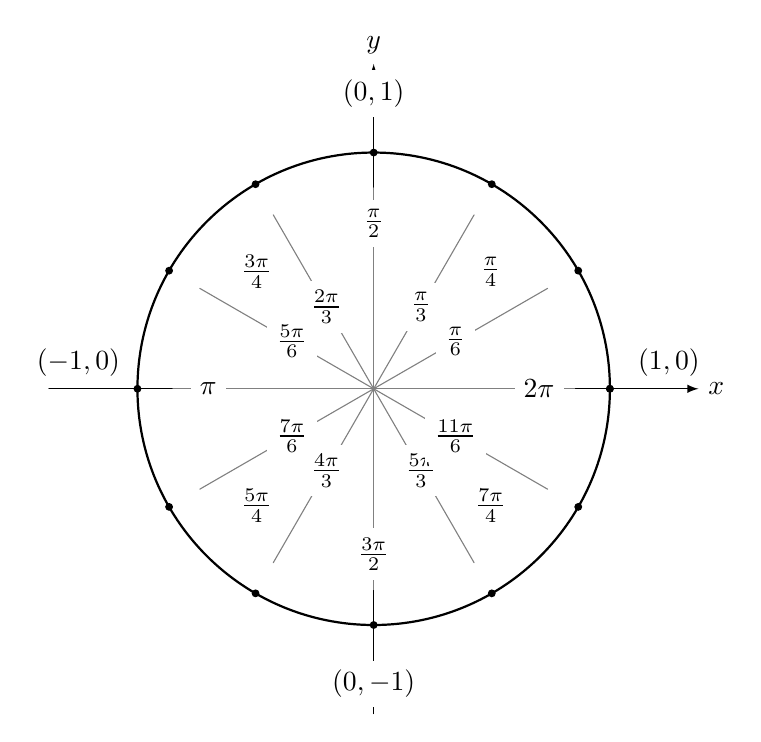
\begin{tikzpicture}[scale=3.0,cap=round,>=latex]
        % draw the coordinates
        \draw[->] (-1.375cm,0cm) -- (1.375cm,0cm) node[right,fill=white] {$x$};
        \draw[->] (0cm,-1.375cm) -- (0cm,1.375cm) node[above,fill=white] {$y$};

        % draw the unit circle
        \draw[thick] (0cm,0cm) circle(1cm);

        \foreach \x in {0,30,...,360} {
                % lines from center to point
                \draw[gray] (0cm,0cm) -- (\x:.85cm);
                % dots at each point
                \filldraw[black] (\x:1cm) circle(0.4pt);
        %         % draw each angle in degrees
        %         \draw (\x:0.6cm) node[fill=white] {$\x^\circ$};
        }

        % draw each angle in radians
        \foreach \x/\xtext in {
            30/\frac{\pi}{6},
            % 45/\frac{\pi}{4},
            60/\frac{\pi}{3},
            % 90/\frac{\pi}{2},
            120/\frac{2\pi}{3},
            % 135/\frac{3\pi}{4},
            150/\frac{5\pi}{6},
            % 180/\pi,
            210/\frac{7\pi}{6},
            % 225/\frac{5\pi}{4},
            240/\frac{4\pi}{3},
            % 270/\frac{3\pi}{2},
            300/\frac{5\pi}{3},
            % 315/\frac{7\pi}{4},
            330/\frac{11\pi}{6}
            % ,
            % 360/2\pi
            }
                \draw (\x:0.4cm) node[fill=white] {$\xtext$};

        \foreach \x/\xtext in {
            % 30/\frac{\pi}{6},
            45/\frac{\pi}{4},
            % 60/\frac{\pi}{3},
            90/\frac{\pi}{2},
            % 120/\frac{2\pi}{3},
            135/\frac{3\pi}{4},
            % 150/\frac{5\pi}{6},
            180/\pi,
            % 210/\frac{7\pi}{6},
            225/\frac{5\pi}{4},
            % 240/\frac{4\pi}{3},
            270/\frac{3\pi}{2},
            % 300/\frac{5\pi}{3},
            315/\frac{7\pi}{4},
            % 330/\frac{11\pi}{6},
            360/2\pi}
                \draw (\x:0.7cm) node[fill=white] {$\xtext$};

        % \foreach \x/\xtext/\y in {
        %     % the coordinates for the first quadrant
        %     30/\frac{\sqrt{3}}{2}/\frac{1}{2},
        %     45/\frac{\sqrt{2}}{2}/\frac{\sqrt{2}}{2},
        %     60/\frac{1}{2}/\frac{\sqrt{3}}{2},
        %     % the coordinates for the second quadrant
        %     150/-\frac{\sqrt{3}}{2}/\frac{1}{2},
        %     135/-\frac{\sqrt{2}}{2}/\frac{\sqrt{2}}{2},
        %     120/-\frac{1}{2}/\frac{\sqrt{3}}{2},
        %     % the coordinates for the third quadrant
        %     210/-\frac{\sqrt{3}}{2}/-\frac{1}{2},
        %     225/-\frac{\sqrt{2}}{2}/-\frac{\sqrt{2}}{2},
        %     240/-\frac{1}{2}/-\frac{\sqrt{3}}{2},
        %     % the coordinates for the fourth quadrant
        %     330/\frac{\sqrt{3}}{2}/-\frac{1}{2},
        %     315/\frac{\sqrt{2}}{2}/-\frac{\sqrt{2}}{2},
        %     300/\frac{1}{2}/-\frac{\sqrt{3}}{2}}
        %         \draw (\x:1.25cm) node[fill=white] {$\left(\xtext,\y\right)$};

        % draw the horizontal and vertical coordinates
        % the placement is better this way
        \draw (-1.25cm,0cm) node[above=1pt] {$(-1,0)$}
              (1.25cm,0cm)  node[above=1pt] {$(1,0)$}
              (0cm,-1.25cm) node[fill=white] {$(0,-1)$}
              (0cm,1.25cm)  node[fill=white] {$(0,1)$};
    \end{tikzpicture}
\begin{center}
    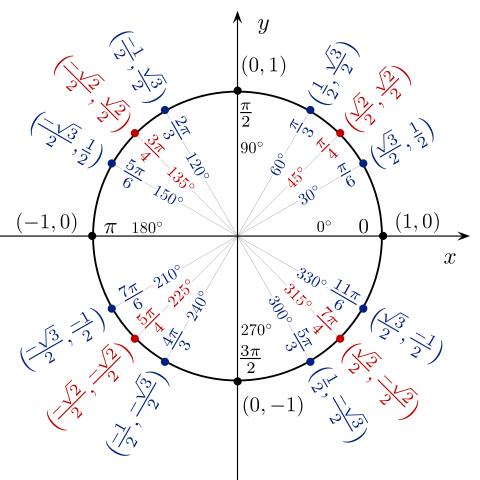
\includegraphics[width=0.48\textwidth]{fig/unit_circle.png}    
\end{center}

\section*{Préfixes Système International}
\begin{center}
\begin{tabular}{lll}
Facteur    & Nom   & Symbol \\\hline\\[-1em]
$10^{6}$   & mega  & M      \\
$10^3$     & kilo  & k      \\
$10^{-3}$  & milli & m      \\
$10^{-6}$  & micro & $\mu$  \\
$10^{-9}$  & nano  & n      \\
$10^{-12}$ & pico  & p     
\end{tabular}
\end{center}

\end{multicols*}

\end{document}
